% !TeX root = ../../main.tex
\begingroup
\ChSixBegin
\emergencystretch=2em
\appendix{T2S2 CHIL}\label{app:ch06}

% CH06-SOURCE-BEGIN
% !TeX root = ../../../../main.tex



This appendix is organized as follows:

\begin{itemize}
    \item \textbf{Appendix~\ref{ch06:apd:subset_ids} (\nameref{ch06:apd:subset_ids}):} PMCID lists for the \texttt{sepsis-40} and \texttt{sepsis-10} annotated subsets.

    \item \textbf{Appendix~\ref{ch06:apd:clinician_quality_review} (\nameref{ch06:apd:clinician_quality_review}):} Expert qualitative review protocol, ranking results, and representative annotation error modes for \texttt{sepsis-10}.

    \item \textbf{Appendix~\ref{ch06:apd:prompt} (\nameref{ch06:apd:prompt}):} Main clinical event--timestamp extraction prompt.

    \item \textbf{Appendix~\ref{ch06:apd:phenotype-prompt} (\nameref{ch06:apd:phenotype-prompt}):} Sepsis-3 phenotyping prompt used for computational labeling.

    \item \textbf{Appendix~\ref{ch06:apd:onset_prompt} (\nameref{ch06:apd:onset_prompt}):} Prompt for sepsis onset timestamp inference.

    \item \textbf{Appendix~\ref{ch06:apd:ltcdf} (\nameref{ch06:apd:ltcdf}):} Derivation and discussion of the area under the log-time curve (AULTC) metric.

    \item \textbf{Appendix~\ref{ch06:apd:pseudo} (\nameref{ch06:apd:pseudo}):} Pseudocode for the recursive best-match procedure used for event alignment.

    \item \textbf{Appendix~\ref{ch06:apd:excerpt} (\nameref{ch06:apd:excerpt}):} Worked examples with manual and LLM annotations, including an illustrative example with finer-grained timing (Appendix~\ref{ch06:apd:fine_example}).

    \item \textbf{Appendix~\ref{ch06:apd:threshold_sweep} (\nameref{ch06:apd:threshold_sweep}):} Sensitivity analysis of the cosine distance matching threshold used to compute event match rate.

    \item \textbf{Appendix~\ref{ch06:apd:add-perf} (\nameref{ch06:apd:add-perf}):} Additional performance analyses and ablation studies.

    \item \textbf{Appendix~\ref{ch06:apd:validation_details} (\nameref{ch06:apd:validation_details}):} Additional details for the hallucination audit, multi-pass self-consistency analysis, and full-corpus cross-model agreement.

    \item \textbf{Appendix~\ref{ch06:apd:error-analysis} (\nameref{ch06:apd:error-analysis}):} Error analysis of event matching and temporal predictions for i2m4 versus \texttt{sepsis-40} performance differences.
\end{itemize}




% !TeX root = ../../../../main.tex
\subsubsection{Annotated PMOA Subsets}
\label{ch06:apd:subset_ids}

The \texttt{sepsis-40} subset contains 40 PMOA case reports with manual clinician annotations, yielding $3,229$ reference clinical events.
The \texttt{sepsis-10} subset is a 10-report subset (801 reference events) of \texttt{sepsis-40} used for clinician annotation quality review, hallucination audit, multi-pass self-consistency, and sepsis onset analysis.


% !TeX root = ../../../../main.tex
\begin{table}[htbp]
\caption{
PMCID composition of the annotated PMOA subsets for \texttt{sepsis-40}.\\
A checkmark indicates membership in \texttt{sepsis-10}.
}\ChSixFloatLabel{ch06:tab:subset_pmcs}
\ChSixTableBodyStart
\begin{ChSixFloatBody}

\centering


\begin{tabular}{lc@{\hspace{3em}}lc}
\toprule
PMCID & \texttt{sepsis-10} & PMCID & \texttt{sepsis-10} \\
\midrule
PMC10037274 &  & PMC10493687 &  \\
PMC3075162  & \checkmark & PMC4421677  &  \\
PMC4929359  &  & PMC5862012  &  \\
PMC6345085  &  & PMC7331532  &  \\
PMC8546416  &  & PMC9355071  & \checkmark \\
PMC10370906 & \checkmark & PMC10556716 & \checkmark \\
PMC3130983  &  & PMC4573216  &  \\
PMC5142474  &  & PMC6059163  &  \\
PMC6441647  &  & PMC7451141  &  \\
PMC8855197  &  & PMC9393191  &  \\
PMC10406025 &  & PMC10629858 & \checkmark \\
PMC3325348  &  & PMC4778217  & \checkmark \\
PMC5721301  &  & PMC6231299  &  \\
PMC6910033  &  & PMC7576661  & \checkmark \\
PMC9136437  & \checkmark & PMC9552858  & \checkmark \\
PMC10480000 &  & PMC2698425  &  \\
PMC4120057  &  & PMC4898175  &  \\
PMC5747955  &  & PMC6238558  & \checkmark \\
PMC7093739  &  & PMC8298783  &  \\
PMC9260376  &  & PMC9647393  &  \\
\bottomrule
\end{tabular}

\end{ChSixFloatBody}
\end{table}

% !TeX root = ../../../../main.tex
\subsubsection{Clinician Annotation Quality Review}
\label{ch06:apd:clinician_quality_review}

\ChSixHeadingOnly
\paragraph{Review protocol}

In addition to the quantitative metrics used in the main evaluation, a physician reviewed extracted timelines for the \texttt{sepsis-10} subset.
For each case report, the clinician assigned: (i) a rank ordering (1 = best, 7 = worst) of the annotations, consisting of the manual annotation and six LLM-generated annotations, and (ii) a categorical assessment (Excellent, Good, Acceptable, or Poor) based on extraction completeness, temporal ordering accuracy, and timing plausibility.
This review provides a qualitative assessment of annotation style and clinical usability, complementing the quantitative event-matching and temporal-alignment metrics reported in the main text.
The reviewed annotation bundle included O1-preview as the OpenAI annotation; replacing GPT-5 which was evaluated separately in the main quantitative results in Table~\ref{ch06:tab:results}.

The clinician review results are reported in Table~\ref{ch06:tab:sep10review}.

\ChSixParagraph{Events requiring temporal reasoning or composition.}
Example: ``passed away'' from ``he was re-admitted to the medical ICU for severe sepsis and multiorgan failure and passed away around 6 months after his initial diagnosis with NHL, despite maintaining a remission status.''
This requires a two-step inference: (1) timing of NHL diagnosis, and (2) adding ``around 6 months'' to that time.
While this is a simple example, more complicated chains of relative timing were noted, sometimes involving other events whose timings are themselves uncertain.
As black-box methods, there is no explicit probabilistic specification for these chains, and empirically we see variable responses.
For this case, the manual annotation is 4383 hours (about 6 months), O1-preview gives 4368 hours (about 6 months), DeepSeek-R1 gives 4032 hours (about 6 months), and Llama 3.3 70B gives 1440 hours (about 2 months); compared to other events the temporal ordering is correct, but the relative timing is off by months.

% !TeX root = ../../../../main.tex
\subsubsection{Annotation Prompt}\label{ch06:apd:prompt}
The main annotation prompt used for clinical finding extraction is shown below. 
Specific components are color-coded to relate them directly to the ablation analysis in Section~\ref{ch06:sec:annotation_results_quantitative} and Table~\ref{ch06:tab:sens}: \textcolor{ChSixDarkPurple}{role-playing instruction} (``You are a physician''), \textcolor{ChSixDarkRed}{conjunction expansion}, and \textcolor{ChSixDarkTeal}{few-shot example}.



\begin{tcolorbox}[breakable,
  colback=teal!5,
  colframe=teal!70!black,
  title=Textual Time Series Generation Prompt,
  boxrule=2pt,
]
\footnotesize
\setlength{\parskip}{1pt}
% \singlespacing
\color{ChSixDarkPurple} You are a physician. 

\color{black}  Extract the clinical events and the related time stamp from the case report. The admission event has timestamp 0. If the event is not available, we treat the event, e.g. current main clinical diagnosis or treatment with timestamp 0. The events happened before event with 0 timestamp have negative time, the ones after the event with 0 timestamp have positive time. The timestamp are in hours. The unit will be omitted when output the result. If there is no temporal information of the event, please use your knowledge and events with temporal expression before and after the events to provide an approximation. We want to predict the future events given the events happened in history. 

\color{ChSixDarkTeal} For example, here is the case report.

An 18-year-old male was admitted to the hospital with a 3-day history of fever and rash. Four weeks ago, he was diagnosed with acne and received the treatment with minocycline, 100 mg daily, for 3 weeks. With increased WBC count, eosinophilia, and systemic involvement, this patient was diagnosed with DRESS syndrome. The fever and rash persisted through admission, and diffuse erythematous or maculopapular eruption with pruritus was present. One day later the patient was discharged.

Let's find the locations of event in the case report, it shows that four weeks ago was the acne diagnosis and start of minocycline treatment, four weeks ago, he was diagnosed with acne and receive treatment. So the event of acne diagnosis and start of minocycline treatment happen four weeks ago, 672 hours, it is before admitted to the hospital, so the time stamp is -672. diffuse erythematous or maculopapular eruption with pruritus was documented on the admission exam, so the time stamp is 0 hours, since it happens right at admission. DRESS syndrome has no specific time, but it should happen soon after admission to the hospital, so we use our clinical judgment to give the diagnosis of DRESS syndrome the timestamp 0. Then the output should look like

18 years old $|$ 0\

male $|$ 0\

admitted to the hospital $|$ 0\

fever $|$ -72\

rash $|$ -72\

acne $|$  -672\

minocycline $|$  -672\

increased WBC count $|$ 0\

eosinophilia$|$ 0\

systemic involvement$|$ 0\

diffuse erythematous or maculopapular eruption$|$ 0\

pruritis $|$ 0\

DRESS syndrome $|$ 0\

fever persisted $|$ 0\

rash persisted $|$ 0\

discharged $|$ 24\ 

\color{ChSixDarkRed}
Separate conjunctive phrases into its component events and assign them the same timestamp (for example, the separation of `fever and rash' into 2 events: `fever' and `rash'). 

\color{black} If the event has duration, assign the event time as the start of the time interval. Attempt to use the text span without modifications except `history of' where applicable. Include all patient events, even if they appear in the discussion; do not omit any events; include termination/discontinuation events; include the pertinent negative findings, like `no shortness of breath' and `denies chest pain'.  Show the events and timestamps in rows, each row has two columns: one column for the event, the other column for the timestamp.  The time is a numeric value in hour unit. The two columns are separated by a pipe `$|$' as a bar-separated file. Skip the title of the table. Reply with the table only. Create a table from the following case: 

\textless \textbackslash end prefix\textgreater

\end{tcolorbox}

% !TeX root = ../../../../main.tex
\subsubsection{Phenotyping Prompt}\label{ch06:apd:phenotype-prompt}
For Sepsis-3 determination, we had a clinician review the discharge summaries and assign each case as meeting the Sepsis-3 definition.  
To develop a computational approach, we constructed a prompt specific to Sepsis-3, which describes the qSOFA procedure for determining a Sepsis-3 diagnosis, and used it as query to Llama-3.1-8B-Instruct (L3.1 8B) and QwQ-32B-Preview (Qwen).  
We used the phenotyping prompt:

\begin{tcolorbox}[breakable,
  colback=yellow!10,
  colframe=orange!80!black,
  title=Phenotyping Prompt,
  boxrule=2pt
]
    {You are an expert physician.}  
    
    {Determine if the patient described in the following case report has either sepsis or septic shock, as defined by the Sepsis-3 criteria, which correspond to having a} 
    
    {(1) suspected or confirmed infection and} 
    
    {(2) blood pressure/respiratory rate/mental status abnormalities.} 
    
    {If the information is not present, use your best judgment based on the information available.} 
    
    {Reply 1 for sepsis, 0 otherwise.} 
    
    {Reply with the number 0 or 1 only in \textbackslash\!boxed\{\textbackslash\!n \boxed{<0 $ or $ 1>} \textbackslash\!n\}with no explanation.}
    
    {Here is the case:} 
    
    {\textless \textbackslash end prefix\textgreater}
\end{tcolorbox}

% !TeX root = ../../../../main.tex
\subsubsection{Sepsis onset inference prompt}
\label{ch06:apd:onset_prompt}
We estimate sepsis onset time relative to admission ($t=0$) using a prompt that requests two onset times: one using qSOFA and one using SOFA-style reasoning when sufficient evidence is available.
The model outputs a two-row bar-separated table with onset timestamps in hours (or NA if criteria are not met).

\begin{tcolorbox}[breakable,
  colback=yellow!10,
  colframe=orange!80!black,
  title=Sepsis Onset Prompt,
  boxrule=2pt
]
    You are an astute physician. 
    
    Determine the time of onset of sepsis using two distinct definitions:
    
    (1) using qSOFA, and 
    
    (2) using SOFA, 
    
    relative to the time of admission which has timestamp 0. 
    
    If the admission time is not available, treat the event, e.g. current main clinical diagnosis or treatment with timestamp 0. The events happened before event with 0 timestamp have negative time, the ones after the event with 0 timestamp have positive time. The timestamps are in hours. The unit will be omitted when output the result. 
    
    If there is no temporal information regarding the onset times, please use your knowledge and events with temporal expression before and after the events to provide an approximation. 
    
    Similarly if the numeric quantities in qSOFA/SOFA are not present, use the available text to infer them as needed.
    
    Show the sepsis onsets and timestamps in rows, each row has two columns: one column for the sepsis definition used (qSOFA or SOFA), the other column for the timestamp. 
    
    The time is a numeric value in hour unit. If criteria is not met, set the time to NA. The two columns are separated by a pipe $|$ as a bar-separated file. Skip the title of the table. Create the table from the following case:
    

    {\textless \textbackslash end prefix\textgreater}

\end{tcolorbox}

% !TeX root = ../../../../main.tex
\subsection{Log-Time Cumulative Distribution Function}
\label{ch06:apd:ltcdf}


Recall the log-time cumulative distribution function is given as follows:

\[
   F(x) = \frac{1}{k} \sum_{i=1}^k \mathbf{1}_{\{x_{(i)} \leq x\}}
\]
where $\mathbf{1}$ is the indicator function.



We compute the AULTC as the area under $F(x)$ from $x = 0$ to $x = \log(1 + S_{\text{max}})$, normalized by $\log(1 + S_{\text{max}})$:
\begin{align*}
\text{AULTC} &= \frac{1}{\log(1 + S_{\text{max}})} \Bigg[ \sum_{i=1}^k (x_{(i)} - x_{(i-1)}) \frac{i}{k} + (\log(1 + S_{\text{max}}) - x_{(k)}) \times 1 \Bigg]
\end{align*}
where $x_{(0)} = 0$.
With this definition, AULTC = 1 indicates that discrepancies are zero (perfect recovery), resulting in maximum area $\log(1 + S_{\text{max}})$, and AULTC = 0 indicates that all discrepancies exceed $S_{\text{max}}$, yielding zero area. 
The code for the AULTC calculation is given in the function \texttt{ecdf\textunderscore auc2(\dots)} in the Supplementary Materials.


\begin{ChSixRemark}
The time unit and cutoff $S_\text{max}$ affect the AULTC calculation, so they must be specified when reporting the AULTC.
\end{ChSixRemark}
Unless otherwise stated, we set $S_{\max}=8760$ hours, corresponding to one year.
This upper limit was chosen because it captures clinically meaningful discrepancies from hours to months while preventing very long-horizon case-history events from dominating the metric.

Because of the $\log(1 + \cdot)$ transformation (rather than the $\log(\cdot)$ transformation which is undefined for zero time-error discrepancy), the discrepancies are non-linearly shifted in the log scale.
The non-linear shift adjusts the relative widths of the step function (particularly for small discrepancies) changing the area calculation.
The cutoff $S_\text{max}$ affects the normalization factor.
Therefore, these values should be chosen based on practicalities for the application.
In our case, we chose hours at the time unit because the only sub-hour descriptions reported were several Apgar scores at the minute-level.

\begin{ChSixRemark}
    The average log-time discrepancy is non-convex.
\end{ChSixRemark}
This can be seen from the observation that the $\log(1+\cdot)$ function is ``spikier'' than the L1 function.
More formally, the log-time discrepancy has a higher curvature around zero error compared to the L1 loss.
Consider the second derivatives of the loss functions with respect to the discrepancies $s = |t^p - t^r|$.
For L1 loss $L_1(s) = s$, the second derivative $\frac{d^2 L_1}{ds^2} = 0$ for $s > 0$.
For the log-time loss, $L_{log}(s) = \log(1 + s)$, the second derivative is $\frac{d^2 L_{log}}{ds^2} = -\frac{1}{(1 + s)^2}$.
At $s = 0$, the second derivative is $-1$, while the second derivative of the L1 loss is $0$.

To provide a simple counterexample, define the average log-time discrepancy is given by:
\[
L(t^p) = \frac{1}{k} \sum_{i=1}^k \log(1 + \min(|t^p_i - t^r_i|, S_{\text{max}}))
\]
To prove that this function is non-convex, we need to show that there exist $t^{p1}, t^{p2}$ and $\lambda \in (0,1)$ such that
\[
L(\lambda t^{p1} + (1-\lambda) t^{p2}) > \lambda L(t^{p1}) + (1-\lambda) L(t^{p2})
\]
Consider the case where $k=1$, $t^r = 0$, and $S_{\text{max}} = 2$.
The loss function is $L(t^p) = \log(1 + \min(|t^p|, 2))$.
Let $t^{p1} = 0$ and $t^{p2} = 3$.
Choose $\lambda = 0.5$.
Then $\lambda t^{p1} + (1-\lambda) t^{p2} = 0.5 \times 0 + 0.5 \times 3 = 1.5$.
Now we evaluate the loss function at these points:
\begin{align*}
L(t^{p1}) &= L(0) = \log(1 + \min(|0|, 2)) = 0 \\
L(t^{p2}) &= L(3) = \log(1 + \min(|3|, 2)) = \\
    & \qquad \log(3) \\
L(\lambda t^{p1} + (1-\lambda) t^{p2}) &= L(1.5) = \log(2.5)
\end{align*}
Now we check the convexity condition:
\[
L(1.5) \leq 0.5 L(0) + 0.5 L(3)
\]
\[
\log(2.5) \leq 0.5 \times 0 + 0.5 \times \log(3)
\]
\[
\log(2.5) \leq \log(\sqrt{3})
\]
Since $2.5 > \sqrt{3} \approx 1.732$, we have $\log(2.5) > \log(\sqrt{3})$.
Therefore,
\[
L(\lambda t^{p1} + (1-\lambda) t^{p2}) > \lambda L(t^{p1}) + (1-\lambda) L(t^{p2})
\]
This proves that the average log-time discrepancy is non-convex.
This remark illustrates the loss form, in case it is considered for optimization/model training rather than for assessment purposes.











% !TeX root = ../../../../main.tex
\subsection{Recursive Best Match Procedure}
\label{ch06:apd:pseudo}
We provide pseudocode for the best match procedure between two lists of strings (Algorithm \ref{ch06:alg:recursive_match}).
For each list, we use the text order, \emph{i.e.}, the order of the events in the annotation files, to break embedding distance ties.
We use the cosine distance for the distance calculation using sentence transformer embeddings from \texttt{S-PubMedBert-MS-MARCO}.


% !TeX root = ../../../../main.tex
\begin{ChSixAlgorithm}[htbp]
\footnotesize
\caption{Recursive Best Match}
\label{ch06:alg:recursive_match}
\SetAlgoLined
\SetKwFunction{ChSixMatchEvents}{MatchEvents}
\SetKwInOut{ChSixInput}{Input}
\SetKwInOut{ChSixOutput}{Output}

\ChSixInput{\quad Two lists: \texttt{ref} (reference events) and \texttt{pred} (predicted events)}
\ChSixOutput{\quad List of best-matching event pairs}
\ChSixMatchEvents{\texttt{ref}, \texttt{pred}} {
    \; 

    \Indp
    \If{ref is empty \textbf{or} pred is empty}{
        \Return{\textbf{[]}}
    }
    Initialize $\text{min\_distance} \gets \infty$\;
    
    Initialize $\text{best\_pair} \gets \text{None}$\;
    
    \ForEach{$r$ \textbf{in} ref}{
        \ForEach{$p$ \textbf{in} pred}{
            $d \gets \text{ComputeDistance}(r, p)$\;
            
            \If{$d < \text{min\_distance}$}{
                $\text{min\_distance} \gets d$\;
                
                $\text{best\_pair} \gets (r, p)$\;
            }\ElseIf{$d = \text{min\_distance}$}{
                $\text{current\_ref\_index} \gets \text{index of } r \text{ in ref}$\;
                
                $\text{current\_pred\_index} \gets \text{index of } p \text{ in pred}$\;
                
                $\text{best\_ref\_index} \gets \text{index of best\_pair.r in ref}$\;
                
                $\text{best\_pred\_index} \gets \text{index of best\_pair.p in pred}$\;
                
                \If{$\text{current\_ref\_index} < \text{best\_ref\_index}$}{
                    $\text{best\_pair} \gets (r, p)$\;
                }\ElseIf{$\text{current\_ref\_index} = \text{best\_ref\_index}$ \textbf{and} $\text{current\_pred\_index} < \text{best\_pred\_index}$}{
                    $\text{best\_pair} \gets (r, p)$\;
                }
            }
        }
    }
    Remove $\text{best\_pair.r}$ from ref\;
    
    Remove $\text{best\_pair.p}$ from pred\;
    
    $\text{result} \gets [\text{best\_pair}] + \text{MatchEvents}
    (\text{ref}, \text{pred})$\;
    
    \Return{$\text{result}$}\;
}
\end{ChSixAlgorithm}






\FloatBarrier

% !TeX root = ../../../../main.tex
\subsection{Example Annotations}\label{ch06:apd:excerpt}
In this section we present an excerpt from PMC10629858, the most recently published case in the \texttt{sepsis-40} dataset \citep{abu2023rare}.
To illustrate the extraction task and performance characteristics of the LLM annotators, we contrast the manual annotations with that of GPT-5, Llama 3.3, and Llama 3.1.


% !TeX root = ../../../../main.tex
\begin{ChSixUncaptionedFigure}
\begin{ChSixFloatBody}

\centering

\begin{tcolorbox}[
  enhanced,
  colback=gray!4,
  colframe=gray!35,
  boxrule=0.4pt,
  arc=2mm,
  left=3mm,right=3mm,top=2mm,bottom=2mm,
]

{\bfseries Excerpt from \cite{abu2023rare}:}


\begin{tcolorbox}[
  enhanced,
  colback=blue!3,
  colframe=blue!60!black,
  title=\textbf{PMC10629858},
  fonttitle=\small,
  % coltitle=black,
  boxrule=0.8pt,
  arc=2mm,
  left=3mm,right=3mm,top=2mm,bottom=2mm
]

\footnotesize

A 57-year-old man recently diagnosed with lepromatous leprosy was confirmed with skin biopsy and had been on treatment (rifampicin/clofazimine/dapsone) for 2 months before admission; he was presented to the hospital with complaints of abdominal distension, constipation, vomiting, and a 10-kg weight loss. On examination, the patient was vitally stable. He had evidence of peripheral lymphadenopathy with a distended abdomen and a positive shifting dullness. A computed tomography scan of his abdomen showed mural thickening of the terminal ileum with significantly enlarged mesenteric lymph nodes, mesenteric fat stranding, and intra-abdominal free fluid, suggesting abdominal granulomatous infection or neoplastic process.

\dots

The patient was planned for consolidation by autologous bone marrow transplant. Unfortunately, with the recurrent bacteremia and sepsis that accompanied the patient’s course due to his immunocompromised state, he was re-admitted to the medical ICU for severe sepsis and multiorgan failure and passed away around 6 months after his initial diagnosis with NHL, despite maintaining a remission status.

\end{tcolorbox}



\begin{minipage}[t]{0.49\textwidth}\vspace{0pt}
 % top-align the pair
\begin{tcolorbox}[ChSix/annobox,title={Manual annotation}]
\ChSixAnnotationTableStyle
\begin{tabular}{>{\raggedright\arraybackslash}p{0.78\textwidth} r}
\toprule
\textbf{Event} & \textbf{Time} \\
\midrule
57-year-old&0 \\
man&0 \\
diagnosed with lepromatous leprosy&-1461 \\
on treatment&-1461 \\
rifampicin&-1461 \\
clofazimine&-1461 \\
dapsone&-1461 \\
presented to the hospital&0 \\
abdominal distension&0 \\
constipation&0 \\
vomiting&0 \\
10-kg weight loss&0 \\
vitally stable&0 \\
peripheral lymphadenopathy&0 \\
distended abdomen&0 \\
positive shifting dullness&0 \\
computed tomography scan of his abdomen&0 \\
mural thickening of the terminal ileum&0 \\
significantly enlarged mesenteric lymph nodes&0 \\
mesenteric fat stranding&0 \\
intra-abdominal free fluid&0 \\
re-admitted to the medical ICU&4383 \\
severe sepsis&4383 \\
multiorgan failure&4383 \\
passed away&4383 \\
\bottomrule
\end{tabular}
\end{tcolorbox}
\end{minipage}
\hfill
\begin{minipage}[t]{0.49\textwidth}\vspace{0pt}

\begin{tcolorbox}[ChSix/annobox,title={GPT-5 annotation}]
\ChSixAnnotationTableStyle
\begin{tabular}{>{\raggedright\arraybackslash}p{0.78\textwidth} r}
\toprule
\textbf{Event} & \textbf{Time} \\
\midrule
57-year-old man & 0 \\
Male & 0 \\
Lepromatous leprosy & -1440 \\
Skin biopsy confirmed lepromatous leprosy & -1440 \\
Started on rifampicin & -1440 \\
Started on clofazimine & -1440 \\
Started on dapsone & -1440 \\
10-kg weight loss & -720 \\
Presented to the hospital & 0 \\
Complaints of abdominal distension & 0 \\
Complaints of constipation & 0 \\
Complaints of vomiting & 0 \\
Patient was vitally stable & 0 \\
Peripheral lymphadenopathy & 0 \\
Distended abdomen & 0 \\
Positive shifting dullness & 0 \\
Computed tomography scan of abdomen & 6 \\
Mural thickening of the terminal ileum & 6 \\
Significantly enlarged mesenteric lymph nodes & 6 \\
Mesenteric fat stranding & 6 \\
Intra-abdominal free fluid & 6 \\
...\\
Bone marrow examination performed & 96 \\
...\\
Re-admitted to the medical ICU & 4380 \\
Severe sepsis & 4380 \\
Multiorgan failure & 4380 \\
Maintaining remission status & 4380 \\
Passed away & 4392 \\
\bottomrule
\end{tabular}
\end{tcolorbox}
\end{minipage}

\end{tcolorbox}

\end{ChSixFloatBody}
\end{ChSixUncaptionedFigure}



% !TeX root = ../../../../main.tex
\begin{ChSixUncaptionedFigure}
\begin{ChSixFloatBody}

\centering
\begin{adjustbox}{max width=\linewidth, max totalheight=0.5\textheight}
\begin{tcolorbox}[ChSix/annopanel]

\begin{minipage}[t]{0.49\textwidth}\vspace{0pt}
   % <-- important
\begin{tcolorbox}[ChSix/annobox,title={DeepSeek-R1-IQ1 annotation}]
\ChSixAnnotationTableStyle
\begin{tabular}{>{\raggedright\arraybackslash}p{0.78\textwidth} r}
\toprule
\textbf{Event} & \textbf{Time} \\
\midrule
57 years old & 0 \\
male & 0 \\
lepromatous leprosy & -1464 \\
skin biopsy & -1464 \\
rifampicin & -1464 \\
clofazimine & -1464 \\
dapsone & -1464 \\
admitted to the hospital & 0 \\
abdominal distension & 0 \\
constipation & 0 \\
vomiting & 0 \\
10-kg weight loss & 0 \\
vital stability & 0 \\
peripheral lymphadenopathy & 0 \\
distended abdomen & 0 \\
positive shifting dullness & 0 \\
computed tomography scan & 0 \\
mural thickening of the terminal ileum & 0 \\
enlarged mesenteric lymph nodes & 0 \\
mesenteric fat stranding & 0 \\
intra-abdominal free fluid & 0 \\
abdominal granulomatous infection or neoplastic process & 0 \\
plan for autologous bone marrow transplant & 0 \\
recurrent bacteremia & 0 \\
sepsis & 0 \\
readmission to medical ICU & 0 \\
severe sepsis & 24 \\
multiorgan failure & 24 \\
passed away & 4032 \\
\bottomrule
\end{tabular}
\end{tcolorbox}
\end{minipage}
\hfill
\begin{minipage}[t]{0.49\textwidth}\vspace{0pt}
   % <-- important
\begin{tcolorbox}[ChSix/annobox,title={Llama-3.3-70B-Instruct annotation}]
\ChSixAnnotationTableStyle
\begin{tabular}{>{\raggedright\arraybackslash}p{0.78\textwidth} r}
\toprule
\textbf{Event} & \textbf{Time} \\
\midrule
57 years old & 0 \\
male & 0 \\
lepromatous leprosy & -720 \\
treatment with rifampicin/clofazimine/dapsone & -720 \\
abdominal distension & 0 \\
constipation & 0 \\
vomiting & 0 \\
10-kg weight loss & 0 \\
peripheral lymphadenopathy & 0 \\
distended abdomen & 0 \\
positive shifting dullness & 0 \\
mural thickening of the terminal ileum & 0 \\
enlarged mesenteric lymph nodes & 0 \\
mesenteric fat stranding & 0 \\
intra-abdominal free fluid & 0 \\
abdominal granulomatous infection & 0 \\
neoplastic process & 0 \\
consolidation by autologous bone marrow transplant & 720 \\
recurrent bacteremia and sepsis & 720 \\
multiorgan failure & 720 \\
death & 1440 \\
\bottomrule
\end{tabular}
\end{tcolorbox}
\end{minipage}

\end{tcolorbox}
\end{adjustbox}

\end{ChSixFloatBody}
\end{ChSixUncaptionedFigure}



% !TeX root = ../../../../main.tex
\begin{ChSixUncaptionedFigure}
\begin{ChSixFloatBody}

\centering
\begin{adjustbox}{max width=\linewidth, max totalheight=0.45\textheight}
\begin{tcolorbox}[ChSix/annopanel]

\begin{minipage}[t]{0.49\textwidth}\vspace{0pt}
   % <-- important
\begin{tcolorbox}[ChSix/annobox,title={Mixtral-8x7B-Instruct v0.1 annotation}]
\ChSixAnnotationTableStyle
\begin{tabular}{>{\raggedright\arraybackslash}p{0.78\textwidth} r}
\toprule
\textbf{Event} & \textbf{Time} \\
\midrule
57 years old& 0 \\
male & 0 \\
recently diagnosed with lepromatous leprosy & -60 \\
on treatment (rifampicin/clofazimine/dapsone) & -60 \\
presented to the hospital & 0 \\
complaints of abdominal distension & 0 \\
complaints of constipation & 0 \\
complaints of vomiting & 0 \\
complaints of 10-kg weight loss & 0 \\
evidence of peripheral lymphadenopathy & 0 \\
distended abdomen & 0 \\
positive shifting dullness & 0 \\
CT showed mural thickening of the terminal ileum & 0 \\
CT showed significantly enlarged mesenteric lymph nodes & 0 \\
CT showed mesenteric fat stranding & 0 \\
CT showed intra-abdominal free fluid & 0 \\
showing a dramatic response to treatment & 0 \\
planned for consolidation by autologous bone marrow transplant & 0 \\
re-admitted to the medical ICU for severe sepsis and multiorgan failure & 0 \\
passed away around 6 months after his initial diagnosis with NHL & 0 \\
despite maintaining a remission status & 0 \\
\bottomrule
\end{tabular}
\end{tcolorbox}
\end{minipage}
\hfill
\begin{minipage}[t]{0.49\textwidth}\vspace{0pt}
   % <-- important
\begin{tcolorbox}[ChSix/annobox,title={Llama-3.1-8B-Instruct annotation}]
\ChSixAnnotationTableStyle
\begin{tabular}{>{\raggedright\arraybackslash}p{0.78\textwidth} r}
\toprule
\textbf{Event} & \textbf{Time} \\
\midrule
18 years old & 0 \\
male & 0 \\
admitted to the hospital & 0 \\
lepromatous leprosy & -720 \\
treatment with rifampicin/clofazimine/dapsone & -720 \\
abdominal distension & -720 \\
constipation & -720 \\
vomiting & -720 \\
weight loss & -720 \\
peripheral lymphadenopathy & -720 \\
distended abdomen & -720 \\
positive shifting dullness & -720 \\
mural thickening of the terminal ileum & -720 \\
enlarged mesenteric lymph nodes & -720 \\
mesenteric fat stranding & -720 \\
intra-abdominal free fluid & -720 \\
abdominal granulomatous infection or neoplastic process & -720 \\
autologous bone marrow transplant & -720 \\
recurrent bacteremia & -720 \\
sepsis & -720 \\
multiorgan failure & -720 \\
passed away & -720 \\
\bottomrule
\end{tabular}
\end{tcolorbox}
\end{minipage}

\end{tcolorbox}
\end{adjustbox}

\end{ChSixFloatBody}
\end{ChSixUncaptionedFigure}




\FloatBarrier
\subsubsection{Additional illustrative example with finer-grained timing}

In this section, we present an additional example representative of case reports with finer-grained temporal detail.
We also show the T2S2 annotation produced by Llama 3.3 alongside the case report to illustrate the extracted timeline for this case report.

\label{ch06:apd:fine_example}

% !TeX root = ../../../../main.tex
\begin{figure}[htbp]
\begin{ChSixFloatBody}

\centering

\begin{tcolorbox}[ChSix/annopanel]

\begin{minipage}[t]{0.48\textwidth}\vspace{0pt}
 % top-align
\begin{tcolorbox}[
  enhanced,
  colback=blue!3,
  colframe=blue!60!black,
  title=\textbf{PMC3184014},
  fonttitle=\small,
  boxrule=0.8pt,
  arc=2mm,
  left=3mm,right=3mm,top=2mm,bottom=2mm
]
\footnotesize\raggedright
A 39-year-old woman with a history of type 2 diabetes, deep vein thrombosis, gastritis, schizophrenia and self-harm presented to the medical admissions unit with a one-week history of a right sub-mammary abscess followed by spreading cellulitis of the breast. On examination she was septic with a pyrexia of 39.2, blood pressure of 127/65 and tachycardia of 110. Examination of the breast revealed widespread cellulitis involving the nipple and sub-mammary area spreading to the axilla. Initial blood tests showed a white cell count of 23.8 (neutrophils 19.9) and CRP of 428. Simple cellulitis was diagnosed by the admitting physicians and she was commenced on parenteral antibiotics and fluid resuscitation. Her condition worsened despite intravenous benzyl penicillin and flucloxacillin. A surgical opinion was sought on day three when she had evidence of synergistic gangrene. The cellulitis had now spread and there were areas of growing necrotic ulceration (Figure~1). Resuscitation was commenced and antibiotic therapy was adjusted to imipenem and clindamycin based on local necrotizing fasciitis guidelines. She was taken to theatre within a few hours where a partial mastectomy was performed and the wound was left open and packed (Figure~2). Postoperatively she remained stable on intensive care. The following day she returned to theatre for further debridement.

The wound was monitored closely and a vacuum dressing was applied to aid healing. Signs of sepsis improved and she returned to the ward on the fifth postoperative day. Nutritional supplements and adequate hydration were continued during her recovery. Secondary closure was performed on day 13 after the initial operation and there was no further breakdown or compromise of the remaining tissues.

Preoperative cultures taken from the ulcers identified a mixture of gram positive and negative bacteria including \textit{Bacteroides} spp. Histology confirmed widespread microscopic changes and abscess formation consistent with gangrene. There was no evidence of malignancy. She was discharged 22 days after admission and follow-up was arranged.
\end{tcolorbox}
\end{minipage}
\hfill
\begin{minipage}[t]{0.48\textwidth}\vspace{0pt}
 % top-align
\begin{tcolorbox}[ChSix/annobox,title={T2S2 annotation}]
\ChSixAnnotationTableStyle
\begin{tabular}{>{\raggedright\arraybackslash}p{0.78\textwidth} r}
\toprule
\textbf{Event} & \textbf{Time} \\
\midrule
39 years old & 0 \\
woman & 0 \\
type 2 diabetes & -168 \\
deep vein thrombosis & -168 \\
gastritis & -168 \\
schizophrenia & -168 \\
self-harm & -168 \\
presented to the medical admissions unit & 0 \\
right sub-mammary abscess & -168 \\
spreading cellulitis of the breast & -168 \\
septic & 0 \\
pyrexia of 39.2 & 0 \\
blood pressure of 127/65 & 0 \\
tachycardia of 110 & 0 \\
widespread cellulitis involving the nipple & 0 \\
cellulitis of the sub-mammary area & 0 \\
cellulitis spreading to the axilla & 0 \\
white cell count of 23.8 & 0 \\
neutrophils of 19.9 & 0 \\
CRP of 428 & 0 \\
diagnosed with simple cellulitis & 0 \\
commenced on parenteral antibiotics & 0 \\
fluid resuscitation & 0 \\
intravenous benzyl penicillin & 0 \\
flucloxacillin & 0 \\
condition worsened & 72 \\
surgical opinion sought & 72 \\
evidence of synergistic gangrene & 72 \\
cellulitis spread & 72 \\
areas of growing necrotic ulceration & 72 \\
resuscitation commenced & 72 \\
antibiotic therapy adjusted to imipenem & 72 \\
antibiotic therapy adjusted to clindamycin & 72 \\
taken to theatre within a few hours & 72 \\
partial mastectomy performed & 72 \\
wound left open and packed & 72 \\
returned to theatre for further debridement & 96 \\
vacuum dressing applied & 96 \\
signs of sepsis improved & 120 \\
returned to the ward & 120 \\
blood markers improved & 168 \\
secondary closure performed & 312 \\
discharged & 528 \\
follow-up arranged & 528 \\
\bottomrule
\end{tabular}
\end{tcolorbox}
\end{minipage}

\end{tcolorbox}




\end{ChSixFloatBody}
\caption{Clinical narrative (left) aligned with temporal T2S2 annotations (right).}\ChSixFloatLabel{ch06:fig:fine-grained-t2s2-annotation}
\end{figure}





\FloatBarrier

% !TeX root = ../../../../main.tex
\subsubsection{Sepsis Event-Matching Threshold Sensitivity}
\label{ch06:apd:threshold_sweep}

Event matching is performed using cosine distance between PubMedBERT embeddings with threshold $\theta = 0.10$ (Section~\ref{ch06:sec:evaluation_methodology_metrics}).
Because the event match recall depends directly on $\theta$, we conducted a sensitivity analysis by sweeping $\theta$ from $0.01$ to $0.50$ in increments of $0.01$ and recomputing event match recall, concordance, and AULTC for each model.


% !TeX root = ../../../../main.tex
\begin{figure}[htbp]
\begin{ChSixFloatBody}

    \centering
    \begin{minipage}[t]{0.48\columnwidth}
        \centering
        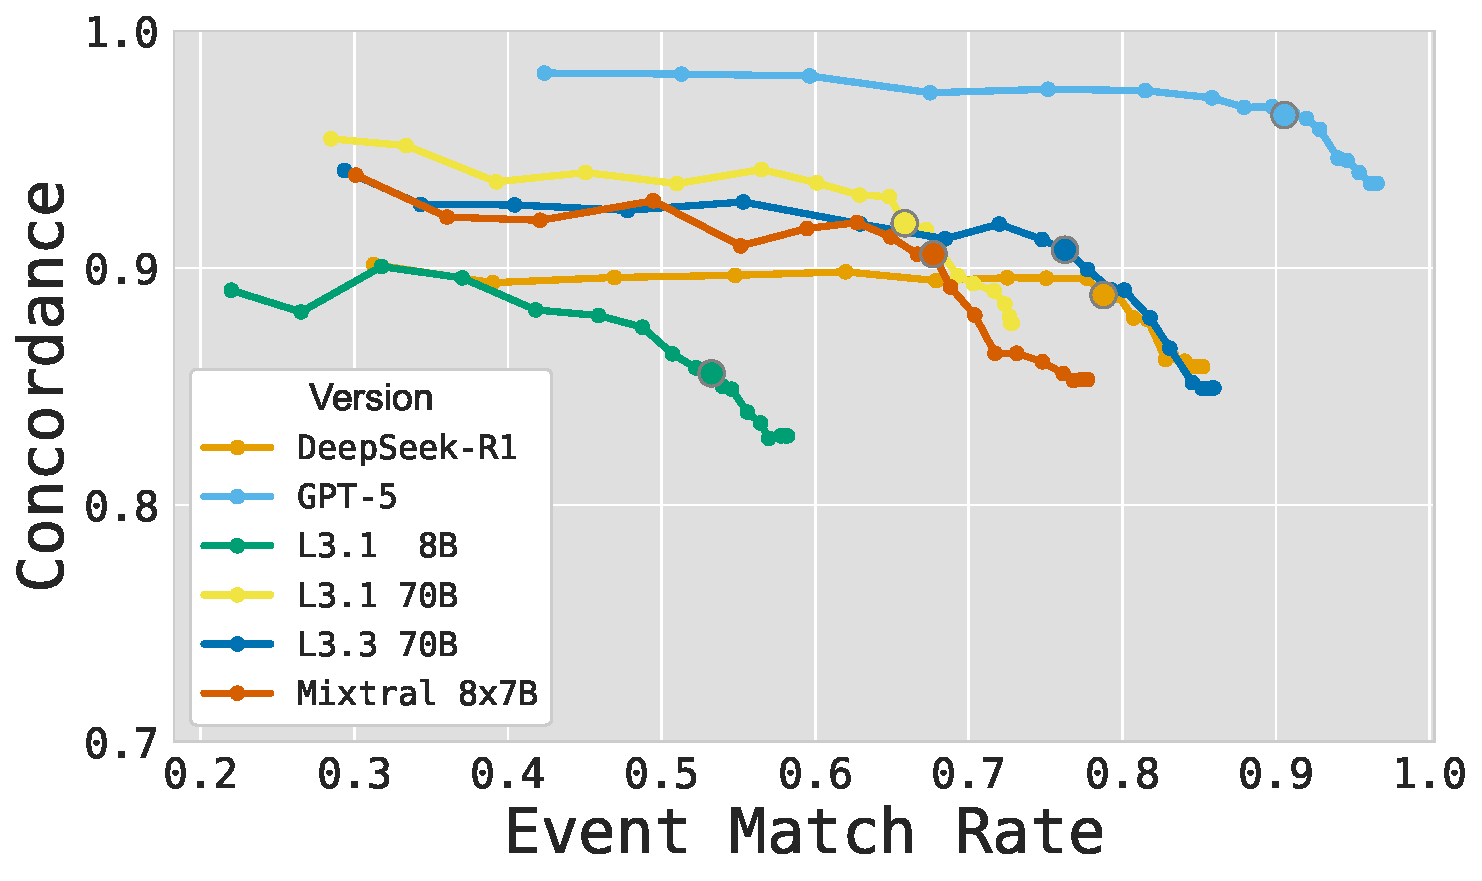
\includegraphics[width=\linewidth]{Appendices/appendix-ch05/sepsis/images/figures/apd_figs/concordance_vs_event_match_rate.pdf}
        
    \end{minipage}\hfill
    \begin{minipage}[t]{0.48\columnwidth}
        \centering
        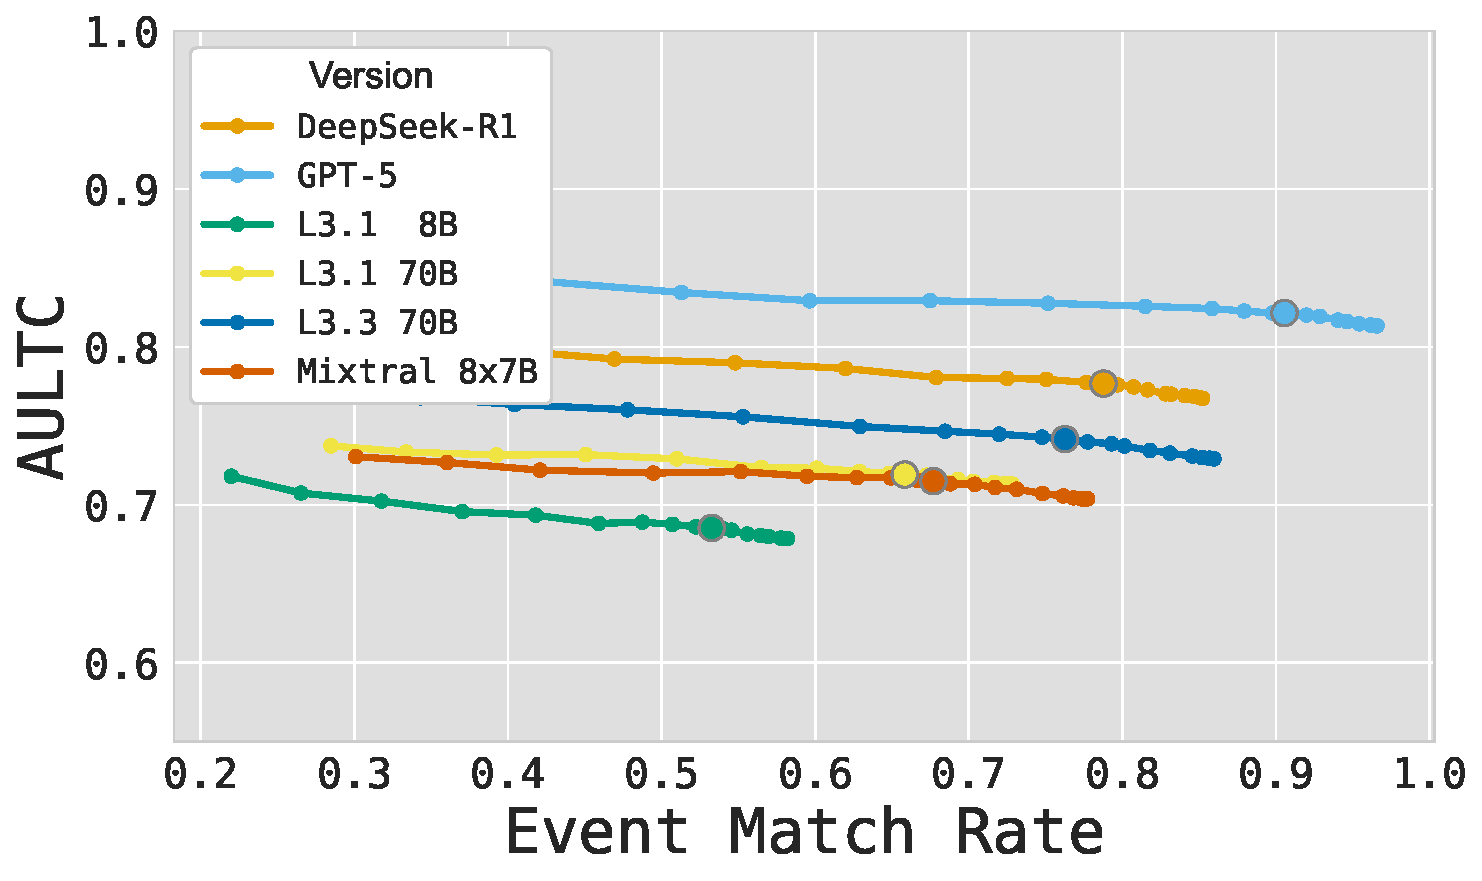
\includegraphics[width=\linewidth]{Appendices/appendix-ch05/sepsis/images/figures/apd_figs/aultc_vs_event_match_rate.pdf}
    \end{minipage}
    
    

\end{ChSixFloatBody}
\caption{Sensitivity of temporal metrics to the cosine distance threshold $\theta$ for the recursive matching heuristic. Left: Concordance versus event match rate obtained by sweeping $\theta$ in increments of $0.01$ over $[0.01, 0.50]$. Right: AULTC versus event match rate under the same sweep. Each point ($\cdot$) corresponds to a distinct threshold value; the solid large circle ($\bullet$) denotes the threshold $\theta = 0.10$ used throughout the paper.}\ChSixFloatLabel{ch06:fig:threshold_sweep}
\ChSixUncaptionedPanelLabel{ch06:fig:threshold_sweep:concordance}
\ChSixUncaptionedPanelLabel{ch06:fig:threshold_sweep:aultc}
\end{figure}


Figure~\ref{ch06:fig:threshold_sweep} shows concordance and AULTC as functions of event match recall induced by varying $\theta$ on the \texttt{sepsis-40} dataset.
As expected, increasing $\theta$ monotonically increases event match recall.
However, beyond a moderate threshold, additional matches correspond to increasingly loose semantic alignments, which degrade temporal metrics.
This produces a characteristic trade-off curve: initial increases in event match recall are accompanied by minimal degradation in concordance and AULTC, followed by a sharper decline once lower-quality matches are admitted.

Across models, we observe a clear ``elbow'' region near $\theta = 0.10$--$0.15$, where event match recall increases modestly while concordance and AULTC remain stable. Beyond this region, particularly past $\theta \approx 0.20$, both concordance and AULTC begin to decline (with concordance drop being more rapid), indicating that additional matches are likely false positive alignments that impair temporal fidelity.

The threshold $\theta = 0.10$ used in the main analysis lies within this elbow region, balancing semantic precision and temporal robustness.
Importantly, relative model ordering remains stable across a wide range of thresholds, suggesting that conclusions regarding comparative performance are not artifacts of a particular cosine distance cutoff of the embeddings.
These results support the use of $\theta = 0.10$ as a conservative and temporally faithful operating point for event matching.





\FloatBarrier

% !TeX root = ../../../../main.tex
\subsection{Additional Performance Analysis}\label{ch06:apd:add-perf}
Here we report performance plots for the \texttt{sepsis-40} ablation analysis and the i2m4 dataset (main analysis and ablation), analogous to Figure \ref{ch06:fig:time-disc}.
Figure \ref{ch06:fig:sep40ablate-time-disc} displays the performance of the Llama 3.3 ablations on \texttt{sepsis-40}.
In terms of match rate, the ablations perform within 5 percent of each other except for the 0-shot and Interval plus Typing (Int+Type) methods.
In the temporal assessment figures we see that, for example, the 0-shot method shows promising temporal performance characteristics, but recall that it suffers from much lower event match rates.
The Interval plus Typing method (Int+Type) shows a similar pattern.
Requesting the interval alone (Interval) results in worse time discrepancy characteristics as compared to the main approach.  


% !TeX root = ../../../../main.tex
\begin{figure}[htbp]
\begin{ChSixFloatBody}

\centering
    \begin{minipage}[t]{0.30\textwidth}
    \centering
    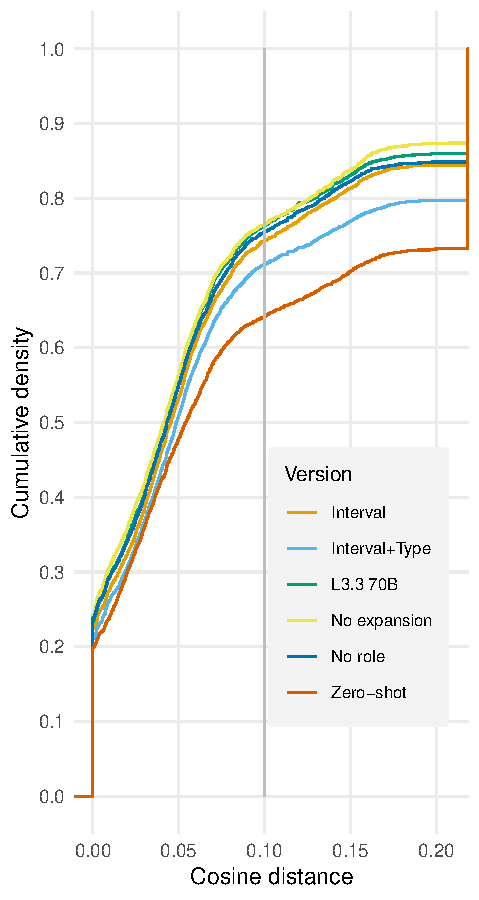
\includegraphics[width=\linewidth, page=1]{Appendices/appendix-ch05/sepsis/images/figures/main_results_figures/figures_sepsis_40_ablations.pdf}
    \end{minipage}
    \begin{minipage}[t]{0.30\textwidth}
    \centering
    \includegraphics[width=\linewidth, page=2]{Appendices/appendix-ch05/sepsis/images/figures/main_results_figures/figures_sepsis_40_ablations.pdf}
    \end{minipage}

    \begin{minipage}[t]{0.30\textwidth}
    \centering
    \includegraphics[width=\linewidth, page=3]{Appendices/appendix-ch05/sepsis/images/figures/main_results_figures/figures_sepsis_40_ablations.pdf}
    \end{minipage}
    \begin{minipage}[t]{0.30\textwidth}
    \centering
    \includegraphics[width=\linewidth, page=4]{Appendices/appendix-ch05/sepsis/images/figures/main_results_figures/figures_sepsis_40_ablations.pdf}
    \end{minipage}
    
    

\end{ChSixFloatBody}
\caption{Event match cumulative distribution function (top left) and  concordance box-plots (top right) for the \texttt{sepsis-40} ablations. 
    Time discrepancy from the manual annotation timestamps among matched events, overall (bottom left) and disaggregated by clinician annotator timestamp (time from presentation, bottom right).}\ChSixFloatLabel{ch06:fig:sep40ablate-time-disc}
\end{figure}


Figures \ref{ch06:fig:i2m4-time-disc} and \ref{ch06:fig:i2m4ablate-time-disc} displays the performance of the models and the Llama 3.3 ablations on the i2m4 dataset.
The match rates and concordances are visibly lower in the i2m4 dataset than in \texttt{sepsis-40}.
Comparing across methods, Llama 3.3 visibly outperforms the Llama 3.1 models in both measures.
Despite the lower match rates and concordances, the time discrepancies in i2m4 were comparatively stronger (AULTC of 0.703).
In terms of time discrepancy, Llama 3.1 70B demonstrate smaller time discrepancies, but at the cost of an event match rate of only 30 percent.
In the ablation analysis of the i2m4 dataset, we observe that the Interval technique performs very similarly to the Llama 3.3 version (unlike in the \texttt{sepsis-40} dataset, where it underperforms markedly with respect to time discrepancy).


% !TeX root = ../../../../main.tex
\begin{figure}[htbp]
\begin{ChSixFloatBody}

\centering
    \begin{minipage}[t]{0.3\textwidth}
    \centering
    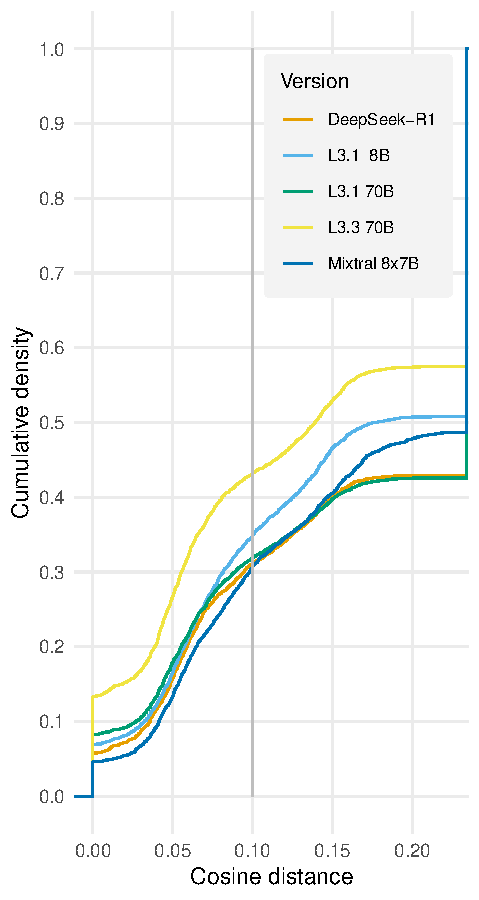
\includegraphics[width=\linewidth, page=1]{Appendices/appendix-ch05/sepsis/images/figures/main_results_figures/figures_i2m4.pdf}
    \end{minipage}
    \begin{minipage}[t]{0.3\textwidth}
    \centering
    \includegraphics[width=\linewidth, page=2]{Appendices/appendix-ch05/sepsis/images/figures/main_results_figures/figures_i2m4.pdf}
    \end{minipage}

    \begin{minipage}[t]{0.3\textwidth}
    \centering
    \includegraphics[width=\linewidth, page=3]{Appendices/appendix-ch05/sepsis/images/figures/main_results_figures/figures_i2m4.pdf}
    \end{minipage}
    \begin{minipage}[t]{0.3\textwidth}
    \centering
    \includegraphics[width=\linewidth, page=4]{Appendices/appendix-ch05/sepsis/images/figures/main_results_figures/figures_i2m4.pdf}
    \end{minipage}
    
    

\end{ChSixFloatBody}
\caption{Event match cumulative distribution function (top left) and  concordance box-plots (top right) for the i2m4 dataset. 
    Time discrepancy from the manual annotation timestamps among matched events, overall (bottom left) and disaggregated by clinician annotator timestamp (time from presentation, bottom right).}\ChSixFloatLabel{ch06:fig:i2m4-time-disc}
\end{figure}



% !TeX root = ../../../../main.tex
\begin{figure}[htbp]
\begin{ChSixFloatBody}

\centering
    \begin{minipage}[t]{0.3\textwidth}
    \centering
    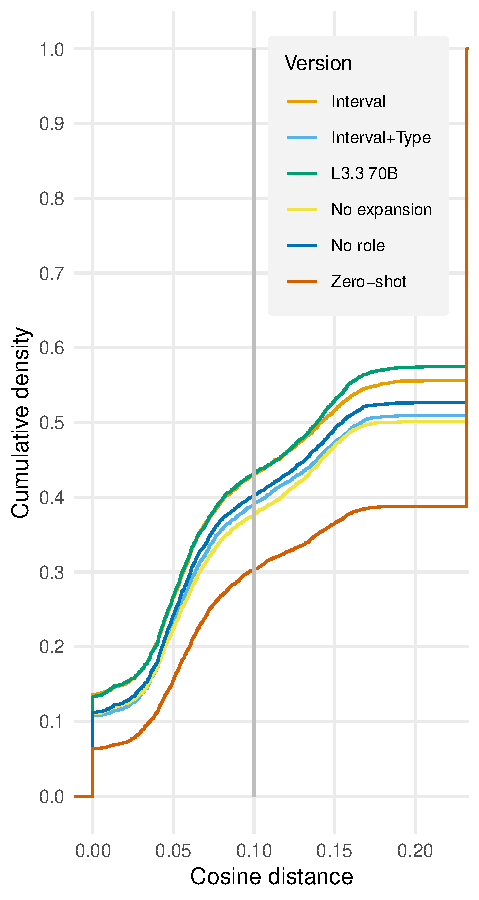
\includegraphics[width=\linewidth, page=1]{Appendices/appendix-ch05/sepsis/images/figures/main_results_figures/figures_i2m4_ablations.pdf}
    \end{minipage}
    \begin{minipage}[t]{0.3\textwidth}
    \centering
    \includegraphics[width=\linewidth, page=2]{Appendices/appendix-ch05/sepsis/images/figures/main_results_figures/figures_i2m4_ablations.pdf}
    \end{minipage}

    \begin{minipage}[t]{0.3\textwidth}
    \centering
    \includegraphics[width=\linewidth, page=3]{Appendices/appendix-ch05/sepsis/images/figures/main_results_figures/figures_i2m4_ablations.pdf}
    \end{minipage}
    \begin{minipage}[t]{0.3\textwidth}
    \centering
    \includegraphics[width=\linewidth, page=4]{Appendices/appendix-ch05/sepsis/images/figures/main_results_figures/figures_i2m4_ablations.pdf}
    \end{minipage}
    
    

\end{ChSixFloatBody}
\caption{Event match cumulative distribution function (top left) and  concordance box-plots (top right) for the i2m4 ablations. 
    Time discrepancy from the manual annotation timestamps among matched events, overall (bottom left) and disaggregated by clinician annotator timestamp (time from presentation, bottom right).}\ChSixFloatLabel{ch06:fig:i2m4ablate-time-disc}
\end{figure}





\FloatBarrier

% !TeX root = ../../../../main.tex
\subsubsection{Grounding and Consistency Protocols}
\label{ch06:apd:validation_details}

This appendix provides details for three validation analyses summarized in Section~\ref{ch06:sec:additional_validation_summary}: the \texttt{sepsis-10} hallucination audit, multi-pass self-consistency analysis, and full-corpus cross-model agreement.
The \texttt{sepsis-10} PMCID composition is provided in Appendix~\ref{ch06:apd:subset_ids}.

\paragraph{Manual hallucination audit}
\label{ch06:apd:hallucination_audit_results}
To directly evaluate whether extracted clinical findings were unsupported by the source text, we performed a two-stage hallucination audit on 10 sampled PMOA case reports.
We audited the DeepSeek-R1 and Llama-3.3-70B-Instruct outputs because they represent two strong model families used for corpus-scale annotation and agreement analyses.
First, we applied automated lexical grounding to each extracted event after light normalization, including removal of prompt-induced prefixes such as ``history of'' or ``treated with''.
The grounding step searched for exact substring matches, ordered token subsequences within a sentence, or unordered token containment in the source report.
Second, all events that could not be automatically grounded were manually reviewed against the original case report to determine whether they represented unsupported hallucinations or valid clinical transformations, such as abbreviation expansion, decomposition of conjunctions, or semantic paraphrasing.
Across DeepSeek-R1 and Llama-3.3-70B-Instruct, this audit covered 1,517 extracted events.
Of these, 1,352 events were grounded automatically by conservative lexical matching, while 165 required manual review because they involved transformations such as abbreviation expansion, conjunction splitting, or semantic paraphrasing.
After manual adjudication of all unresolved cases against the original reports, we identified \textbf{0} hallucinated events (Table~\ref{ch06:tab:hallucination_audit}).
This result does not prove that hallucinations never occur in the full corpus, but it provides direct evidence that under the extractive formulation used here, unsupported event fabrication was not observed in the audited subset.


% !TeX root = ../../../../main.tex
\begin{table}[htbp]
\caption{Manual hallucination audit on 10 PMOA case reports. Automated lexical grounding used exact substring, ordered token subsequence, or unordered token containment after normalization. Events not grounded automatically were manually reviewed against the source report. Manual review identified 0 hallucinated events.}\ChSixFloatLabel{ch06:tab:hallucination_audit}
\ChSixTableBodyStart
\begin{ChSixFloatBody}

\centering
\small


\begin{adjustbox}{max width=\textwidth}
\begin{tabular}{lrrrrrr}
\toprule
& \multicolumn{3}{c}{DeepSeek-R1} & \multicolumn{3}{c}{L3.3 70B} \\
\cmidrule(lr){2-4}\cmidrule(lr){5-7}
PMOA case ID & Events & Auto-grounded & Manual review & Events & Auto-grounded & Manual review \\
\midrule
PMC10370906 & 59 & 51 & 8 & 73 & 72 & 1 \\
PMC10556716 & 107 & 95 & 12 & 115 & 110 & 5 \\
PMC10629858 & 77 & 73 & 4 & 63 & 61 & 2 \\
PMC3075162 & 87 & 77 & 10 & 77 & 74 & 3 \\
PMC4778217 & 65 & 63 & 2 & 63 & 60 & 3 \\
PMC6238558 & 70 & 66 & 4 & 71 & 64 & 7 \\
PMC7576661 & 45 & 41 & 4 & 54 & 45 & 9 \\
PMC9136437 & 69 & 59 & 10 & 125 & 124 & 1 \\
PMC9355071 & 58 & 43 & 15 & 57 & 45 & 12 \\
PMC9552858 & 101 & 63 & 38 & 81 & 66 & 15 \\
\midrule
Total & 738 & 631 & 107 & 779 & 721 & 58 \\
\bottomrule
\end{tabular}
\end{adjustbox}

\end{ChSixFloatBody}
\end{table}


\ChSixParagraph{Hallucination audit interpretation}
The hallucination audit was designed to distinguish unsupported event fabrication from valid clinical transformations.
Events requiring manual review were not automatically considered hallucinations, because T2S2 annotations may legitimately expand abbreviations, split conjunctions, or paraphrase source text into standalone clinical findings.
For example, an extracted event such as ``PET/CT'' may correspond to the source phrase ``positron emission tomography/computed tomography,'' and an extracted event such as ``clinical deterioration'' may correspond to the source phrase ``deteriorated clinically.''
Similarly, medication stop events may require combining a causal statement with a later phrase indicating that multiple drugs were stopped.
After manual review of all unresolved cases in the audited subset, no unsupported events were identified.


\FloatBarrier
\paragraph{Multi-pass self-consistency}
\label{ch06:apd:self_consistency_results}
To assess robustness across generations, we re-annotated the same 10 reports used in the hallucination audit using five random seeds for DeepSeek-R1, Llama-3.3-70B-Instruct, OpenAI O1-preview, and GPT-5.
For each model, Run 1 was treated as the within-model reference and Runs 2--5 were compared against it.
All four evaluated models showed high self-consistency across repeated generations (Table~\ref{ch06:tab:self_consistency}).
GPT-5 and Llama 3.3 had particularly high event match recall values across runs, while DeepSeek-R1 and O1-preview also showed stable temporal ordering and AULTC.
These results suggest that the extracted timelines are not highly sensitive to random seed variation and that the pipeline does not exhibit the low-consistency behavior often associated with hallucinated or unstable generations.


% !TeX root = ../../../../main.tex
\begin{table}[htbp]
\ChSixUseRaggedCaption
\caption{Multi-pass self-consistency across five random seeds on the 10-report hallucination-audit subset. Run 1 is used as the within-model reference; Runs 2--5 are compared against Run 1.}\ChSixFloatLabel{ch06:tab:self_consistency}
\ChSixTableBodyStart
\begin{ChSixFloatBody}

\centering
\small


\begin{adjustbox}{max width=\textwidth}
\begin{tabular}{llccc}
\toprule
Model & Run & Event match recall & Concordance & AULTC \\
\midrule
DeepSeek-R1 & Run 2 & 0.852 & 0.907 & 0.878 \\
DeepSeek-R1 & Run 3 & 0.836 & 0.890 & 0.835 \\
DeepSeek-R1 & Run 4 & 0.839 & 0.892 & 0.860 \\
DeepSeek-R1 & Run 5 & 0.821 & 0.878 & 0.852 \\
\midrule
L3.3 70B & Run 2 & 0.943 & 1.000 & 0.708 \\
L3.3 70B & Run 3 & 0.937 & 1.000 & 0.753 \\
L3.3 70B & Run 4 & 0.954 & 1.000 & 0.735 \\
L3.3 70B & Run 5 & 0.953 & 1.000 & 0.755 \\
\midrule
O1-preview & Run 2 & 0.838 & 0.942 & 0.828 \\
O1-preview & Run 3 & 0.852 & 0.972 & 0.852 \\
O1-preview & Run 4 & 0.855 & 0.965 & 0.840 \\
O1-preview & Run 5 & 0.847 & 0.941 & 0.847 \\
\midrule
GPT-5 & Run 2 & 0.935 & 0.924 & 0.860 \\
GPT-5 & Run 3 & 0.918 & 0.958 & 0.878 \\
GPT-5 & Run 4 & 0.911 & 0.942 & 0.863 \\
GPT-5 & Run 5 & 0.934 & 0.922 & 0.856 \\
\bottomrule
\end{tabular}
\end{adjustbox}

\end{ChSixFloatBody}
\end{table}



\ChSixParagraph{Interpretation of self-consistency}
The self-consistency analysis evaluates stability of the extraction process across repeated generations.
High self-consistency does not prove clinical correctness, but low self-consistency would indicate that extracted timelines are sensitive to sampling noise and therefore less reliable as corpus annotations.
The observed consistency across DeepSeek-R1, Llama 3.3, O1-preview, and GPT-5 suggests that the prompt and extraction schema induce stable behavior across repeated runs.


\FloatBarrier
\paragraph{Full-corpus cross-model agreement}
\label{ch06:apd:full_corpus_agreement_results}
Finally, we evaluated cross-model agreement across all 2,139 T2S2 reports to assess extraction consistency beyond the manually annotated subset.
Treating DeepSeek-R1 as a proxy reference, Llama-3.3-70B-Instruct achieved an event match recall of 0.79, concordance of 0.87, and AULTC of 0.83 across the full corpus (Table~\ref{ch06:tab:full_corpus_agreement}).
Because these models differ in architecture and training, this agreement provides a scalable reliability signal that the extracted trajectories are systematic and reproducible across model families.
We emphasize that this analysis is not a substitute for clinical adjudication, but rather a corpus-scale agreement check complementing the gold-standard \texttt{sepsis-40} evaluation, clinician--clinician agreement, hallucination audit, and self-consistency results.


% !TeX root = ../../../../main.tex
\begin{table}[htbp]
\caption{Full-corpus cross-model agreement across all 2,139 T2S2 reports. DeepSeek-R1 is treated as the proxy reference.}\ChSixFloatLabel{ch06:tab:full_corpus_agreement}
\ChSixTableBodyStart
\begin{ChSixFloatBody}

\centering
\small


\begin{adjustbox}{max width=\columnwidth}
\begin{tabular}{lccc}
\toprule
Model comparison & Event match recall & Concordance & AULTC \\
\midrule
L3.3 70B vs.\ DeepSeek-R1 & 0.79 & 0.87 & 0.83 \\
\bottomrule
\end{tabular}
\end{adjustbox}

\end{ChSixFloatBody}
\end{table}



\ChSixParagraph{Interpretation of full-corpus cross-model agreement}
Full-corpus cross-model agreement complements gold-standard evaluation by estimating whether two independent model families produce similar event--time trajectories across all 2,139 reports.
This analysis is not intended to replace clinician adjudication and cannot identify all shared model errors.
However, strong agreement across model families provides evidence that the extraction behavior is systematic at corpus scale rather than being driven by isolated idiosyncratic outputs from a single model.




\FloatBarrier

% !TeX root = ../../../../main.tex

\subsubsection{Event Counts and Annotation Schema}\label{ch06:apd:error-analysis}
To investigate the discrepancies in event match recall between the i2m4 and \texttt{sepsis-10} datasets, we analyzed the datasets' structure and examined model performance using Llama 3.3 as a representative model, as the pattern of differences observed across datasets was consistent for all models.

\ChSixParagraph{Overview of Clinical Event Identification.}
For the i2m4 dataset, manual annotations by clinicians identified an average of $195\pm94$ clinical events per report across $20$ case reports, compared to $80\pm28$ clinical events per report for \texttt{sepsis-10} across $10$ case reports.
Llama 3.3 identified an average of $120\pm61$ clinical events for i2m4 and $78\pm24$ clinical events for \texttt{sepsis-10}.
These results highlight a systematic bias of under-identification of clinical events in i2m4 compared to \texttt{sepsis-10} by Llama 3.3.

Additionally, the i2m4 dataset contains approximately $2.4\times$ more clinical events per report on average than \texttt{sepsis-10}, as annotated by the clinician, with a much larger variance in event counts across reports.
This heterogeneity reflects structural differences in the datasets: i2m4 reports often include a large number of structured entries, whereas \texttt{sepsis-10} reports are only made-up of free text.
Llama 3.3 over-identified clinical events (i.e., predicted more events than the manual annotators) in $15\%$ of i2m4 reports, while under-identifying events in $85\%$ of i2m4 reports.
For \texttt{sepsis-10}, the model showed a more balanced distribution, over-identifying and under-identifying events in $50\%$ of reports each (Table~\ref{ch06:tab:event_identification_bias}).
These patterns suggest that the higher density and variability of clinical events in i2m4 pose a greater challenge for Llama 3.3.






% !TeX root = ../../../../main.tex
\begin{table}[htbp]
\caption{Proportion of reports where Llama 3.3 over- or under-identified clinical events compared to manual annotations. i2m4 shows a strong bias toward under-identification, whereas \texttt{sepsis-10} has a more balanced distribution.}\ChSixFloatLabel{ch06:tab:event_identification_bias}
\ChSixTableBodyStart
\begin{ChSixFloatBody}

\setlength{\tabcolsep}{4pt}
\centering
\begin{tabular}{|l|c|c|}
\hline
\textbf{Dataset} & \makecell{\textbf{\% Reports} \\ \textbf{Over-Identified}} & \makecell{\textbf{\% Reports} \\ \textbf{Under-Identified}} \\ \hline
\textbf{i2m4}    & 15\%                                & 85\%                                 \\ \hline
\textbf{\texttt{sepsis-10}} & 50\%                              & 50\%                                 \\ \hline
\end{tabular}



\end{ChSixFloatBody}
\end{table}


\ChSixParagraph{Dataset Structure Differences.}
The differences in dataset structure between i2m4 and \texttt{sepsis-10} are also evident in the length of clinical events.
As shown in Table~\ref{ch06:tab:character_length}, the manually annotated clinical events in i2m4 are significantly shorter, averaging $10\pm7$ characters, compared to $28\pm16$ characters in \texttt{sepsis-10}.
This reflects the structured nature of i2m4 reports, which often include tables with abbreviations (e.g., ``K'' for Potassium, ``Na'' for Sodium).



% !TeX root = ../../../../main.tex
\begin{table}[htbp]
\caption{Average length of clinical events in characters for both datasets. Manual annotations in i2m4 are significantly shorter due to frequent abbreviations and structured text from MIMIC tables, while Llama 3.3 generates events of comparable length across datasets.}\ChSixFloatLabel{ch06:tab:character_length}
\ChSixTableBodyStart
\begin{ChSixFloatBody}

\centering
\begin{tabular}{|l|c|c|}
\hline
\textbf{Dataset} & \textbf{Manual Annotator} & \textbf{Llama 3.3} \\ \hline
\textbf{i2m4}    & $10\pm7 $                              & $17\pm14$                        \\ \hline
\textbf{\texttt{sepsis-10}} & $28\pm16$                            & $21\pm13$                        \\ \hline
\end{tabular}



\end{ChSixFloatBody}
\end{table}


Llama 3.3-generated clinical events are of similar length across datasets, with averages of $17\pm14$ characters for i2m4 and $21\pm13$ characters for \texttt{sepsis-10}.
This consistency suggests that Llama 3.3 applies similar generative behavior across datasets, often producing expanded forms of abbreviations in i2m4.
While this generative behavior mitigates variability in Llama 3.3 outputs, it creates a mismatch with the shorter, more concise manual annotations in i2m4.
This mismatch can then contribute to higher cosine distances between embeddings, lowering the event match recall for i2m4.

% CH06-SOURCE-END
\clearpage
\endgroup
